\documentclass[tikz,border=10pt]{standalone}
\usepackage{pgfplots}
\usepackage{tikz}
\usepackage{amsmath}

\begin{document}
\centering
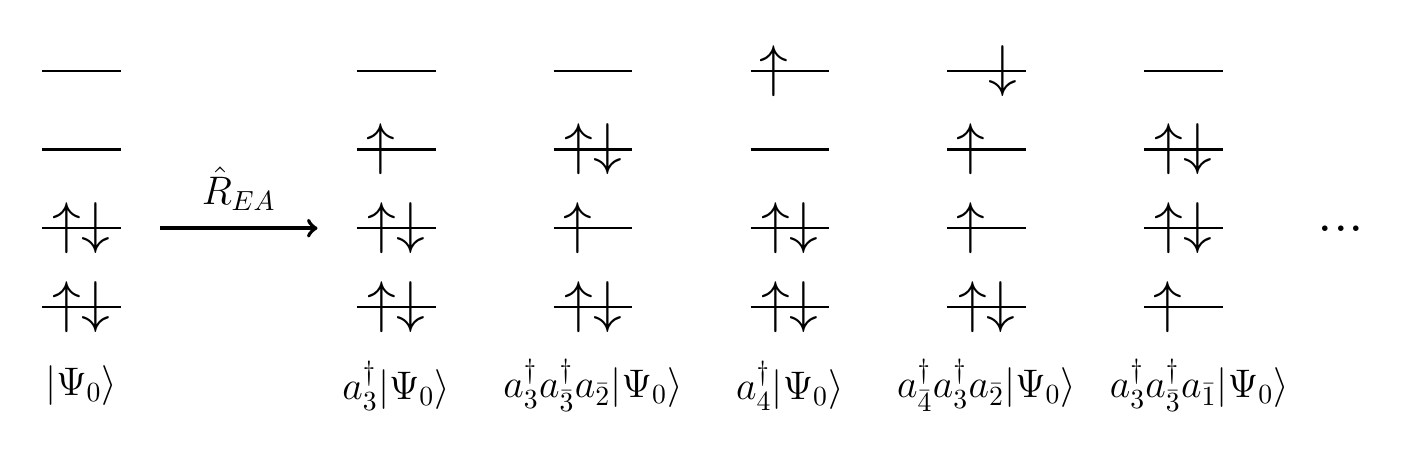
\begin{tikzpicture}
    \huge
    % Define styles
    \tikzset{
        level/.style={thick},
        arrow/.style={->, thick},
        label/.style={font=\small}
    }

    % Draw CC wavefunction levels (left)
    \draw[level] (-2,3) -- (-1,3); 
    \draw[level] (-2,2) -- (-1,2); 
    \draw[level] (-2,2) -- (-1,2); 
    \draw[level] (-2,1) -- (-1,1);
    \draw[level] (-2,0) -- (-1,0);
    % Draw electron occupancies for CC
    \node at (-1.5,0) {\(\uparrow\downarrow\)};
    \node at (-1.5,1) {\(\uparrow\downarrow\)};
    % Label CC wavefunction
    \node[label] at (-1.5,-1) {\Large\(|\Psi_{\text{0}}\rangle\)};    

    % Draw transition arrow and label
    \draw [->,line width=0.5mm] (-0.5,1) -- (1.5,1);
    \node[label] at (0.5,1.5) {\Large\(\hat{R}_{EA}\)};

    % Draw EA wavefunction levels (right)
    \draw[level] (2,3) -- (3,3);
    \draw[level] (2,2) -- (3,2);
    \draw[level] (2,1) -- (3,1);
    \draw[level] (2,0) -- (3,0);
    % Draw electron occupancies for EA
    \node at (2.3,2) {\(\uparrow\)};
    \node at (2.5,0) {\(\uparrow\downarrow\)};
    \node at (2.5,1) {\(\uparrow\downarrow\)};
    % Label EA wavefunction
    \node[label] at (2.5,-1) {\Large\(a^\dagger_3|\Psi_{\text{0}}\rangle\)};

    % Draw EA2 wavefunction levels (right)
    \draw[level] (4.5,3) -- (5.5,3);
    \draw[level] (4.5,2) -- (5.5,2);
    \draw[level] (4.5,1) -- (5.5,1);
    \draw[level] (4.5,0) -- (5.5,0);
    % Draw electron occupancies for EA
    \node at (5,2) {\(\uparrow\downarrow\)};
    \node at (4.8,1) {\(\uparrow\)};
    \node at (5,0) {\(\uparrow\downarrow\)};
    % Label EA wavefunction
    \node[label] at (5,-1) {\Large\(a^\dagger_3 a^\dagger_{\bar{3}} a_{\bar{2}}|\Psi_{\text{0}}\rangle\)};

    % Draw EA3 wavefunction levels (right)
    \draw[level] (7,3) -- (8,3);
    \draw[level] (7,2) -- (8,2);
    \draw[level] (7,1) -- (8,1);
    \draw[level] (7,0) -- (8,0);
    % Draw electron occupancies for EA
    \node at (7.3,3) {\(\uparrow\)};
    \node at (7.5,0) {\(\uparrow\downarrow\)};
    \node at (7.5,1) {\(\uparrow\downarrow\)};
    % Label EA wavefunction
    \node[label] at (7.5,-1) {\Large\(a^\dagger_4|\Psi_{\text{0}}\rangle\)};

    % Draw EA wavefunction levels (right)
    \draw[level] (9.5,3) -- (10.5,3);
    \draw[level] (9.5,2) -- (10.5,2);
    \draw[level] (9.5,1) -- (10.5,1);
    \draw[level] (9.5,0) -- (10.5,0);
    % Draw electron occupancies for EA
    \node at (10.2,3) {\(\downarrow\)};
    \node at (9.8,2) {\(\uparrow\)};
    \node at (9.8,1) {\(\uparrow\)};
    \node at (10,0) {\(\uparrow\downarrow\)};
    % Label EA wavefunction
    \node[label] at (10,-1) {\Large\(a^\dagger_{\bar{4}} a^\dagger_3 a_{\bar{2}}|\Psi_{\text{0}}\rangle\)};

    % Draw EA2 wavefunction levels (right)
    \draw[level] (12,3) -- (13,3);
    \draw[level] (12,2) -- (13,2);
    \draw[level] (12,1) -- (13,1);
    \draw[level] (12,0) -- (13,0);
    % Draw electron occupancies for EA
    \node at (12.5,2) {\(\uparrow\downarrow\)};
    \node at (12.5,1) {\(\uparrow\downarrow\)};
    \node at (12.3,0) {\(\uparrow\)};
    % Label EA wavefunction
    \node[label] at (12.7,-1) {\Large\(a^\dagger_3 a^\dagger_{\bar{3}} a_{\bar{1}}|\Psi_{\text{0}}\rangle\)};    

    \node[label] at (14.5,1) {\huge\(...\)}; 
\end{tikzpicture}
\end{document}